\documentclass[12pt]{article}
\usepackage{graphicx,psfrag,amsfonts,float,mathbbol,xcolor}
\usepackage{amsmath}
\usepackage{mathtools}
\usepackage{IEEEtrantools}
\usepackage[letterpaper, left=1in, top=1in, right=1in, bottom=1in,nohead,includefoot, verbose, ignoremp]{geometry}
\newcommand*\needsparaphrased{\color{red}}
\newcommand*\paraphrase{\color{orange}}
\newcommand*\outlineskeleton{\color{green}}
\newcommand{\bfeps}{\mbox{\boldmath $\epsilon$}}
\newcommand{\bfgamma}{\mbox{\boldmath $\gamma$}}
\newcommand{\bflam}{\mbox{\boldmath $\lambda$}}
\newcommand{\bfphi}{\mbox{\boldmath $\phi$}}
\newcommand{\bfsigma}{\mbox{\boldmath $\sigma$}}
\newcommand{\bfbeta}{\mbox{\boldmath $\beta$}}
\newcommand{\bfalpha}{\mbox{\boldmath $\alpha$}}
\newcommand{\bfe}{\mbox{\boldmath $e$}}
\newcommand{\bff}{\mbox{\boldmath $f$}}
\newcommand{\bft}{\mbox{\boldmath $t$}}
\newcommand{\bfo}{\mbox{\boldmath $0$}}
\newcommand{\bfO}{\mbox{\boldmath $O$}}
\newcommand{\bfx}{\mbox{\boldmath $x$}}
\newcommand{\bfX}{\mbox{\boldmath $X$}}
\newcommand{\bfz}{\mbox{\boldmath $z$}}


\newcommand{\bfm}{\mbox{\boldmath $m}}
\newcommand{\bfy}{\mbox{\boldmath $y$}}
\newcommand{\bfd}{\mbox{\boldmath $d$}}
\newcommand{\bfc}{\mbox{\boldmath $c$}}
\newcommand{\bfa}{\mbox{\boldmath $a$}}
\newcommand{\bfb}{\mbox{\boldmath $b$}}
\newcommand{\bfY}{\mbox{\boldmath $Y$}}
\newcommand{\bfS}{\mbox{\boldmath $S$}}
\newcommand{\bfZ}{\mbox{\boldmath $Z$}}
\newcommand{\cardT}{\vert \mathcal{T} \vert}
\newenvironment{theorem}[1][Theorem]{\begin{trivlist}
\item[\hskip \labelsep {\bfseries #1}]}{\end{trivlist}}
\newenvironment{corollary}[1][Corollary]{\begin{trivlist}
\item[\hskip \labelsep {\bfseries #1}]}{\end{trivlist}}
\newenvironment{proposition}[1][Proposition]{\begin{trivlist}
\item[\hskip \labelsep {\bfseries #1}]}{\end{trivlist}}
\newenvironment{definition}[1][Definition]{\begin{trivlist}
\item[\hskip \labelsep {\bfseries #1}]}{\end{trivlist}}

\def\bL{\mathbf{L}}


 \begin{document}

\nocite{*}
%\chapter{Varying Coefficient Models for Longitudinal Data}
%\label{VCmodelsForLongitudinalData.ch}

\section{Nonparametric extensions of the classical linear model}

The classical linear model expresses the influence of covariates $X_1, X_2, \dots, X_p$ on the response variable $Y$ via 

\begin{equation} \label{eq:classical_linear_model}
Y = \beta_1 X_1 + \beta_2 X_2 + \dots + \beta_p X_p 
\end{equation}

While linearity is a convenient artifact of specifying model \ref{eq:classical_linear_model}, the world is full of nonlinear phenomena such as limit cycles and jump resonance. Consequently, nonlinearity must be a modeling consideration to adequately characterize many of the natural underlying mechanisms that generate data. The nonparametric regression model has been widely used in various applications due to its ability to characterize structure in data that linear and other parametric models fail to adequately represent. However, a serious drawback to the general nonparametric model is the ?curse of dimensionality? phenomenon, a term which refers to the fact that the convergence rate of nonparametric smoothing estimators becomes rather slow when the estimation target is a general function of a large number of variables without additional structures. Many efforts have been made to impose structure on the regression function to alleviate this issue, which is broadly described as dimension reduction. Some approaches to restricting the general nonparametric model include: (generalized) additive models \cite{chen1993nonlinear}\cite{hastie1990generalized}, \cite{hastie1986generalized}, Sperlich, Tjostheim \& Yang 2002, Stone 1985), partially linear models \cite{hardle2007partially}, \cite{zeger1994semiparametric}, varying coefficient models \cite{hastie1993varying}, Fan \& Zhang, 1999), and their hybrids  (Carroll et al., 1997; Fan et al., 1998; Heckman et al., 1998), among others.

An immediate problem of departing from linearity is the need for a class of well-parameterized nonlinear models that are simple yet sufficient in handling most nonlinear phenomena observed in practice. Because there is no unified theory applicable to all nonlinear models, this problem is a difficult one. The main difficulty is that unlike linear models where the functions involved can be treated fairly systematically, the set of all nonlinear models is so broad that systematic treatment is infeasible. The expansiveness of the class of nonlinear models is due to both the innumerable nonlinear functions as well as the different structures within a given class of functions. 
 
Varying coefficient models are a particularly attractive extension of the classical linear model. The appeal of this model is that, by allowing regression coefficients to depend on a smoothing parameter $Z$, the modeling bias can significantly be reduced while avoiding the``curse of dimensionality''. Another advantage of this model is its interpretability, and this model structure arises naturally when one is interested in exploring how regression coefficients change over different groups, such as age. The mean function of the response $Y$ take the form

\subsection{{\outlineskeleton Extensions of linear models which are special cases of models in \ref{univariate_VC_models},\ref{multivariate_VC_models},\ref{extended_VC_models}}}
To illustrate the flexibility of the varying coefficient model, we examine some models that may be expressed as special cases, first considering the general nonparametric modeling literature. 


\section{{\outlineskeleton VC Models with a Univariate Smoothing Variable}} \label{univariate_VC_models}

\begin{equation} \label{eq:VC_mean_function_single_smoothing_covariate}
E\left(Y \vert \bfX=\bfx,\;Z = z \right) = x_1\beta_1\left(z\right) + \dots  + x_p\beta_p\left(z\right)
\end{equation}
\noindent
where $\bfX = \left(X_1, X_2, \dots, X_p\right)^T$ and $Z$ are covariates and $\bfbeta\left(z\right) = \left( \beta_0\left(z\right), \beta_1\left(z\right),\dots,\beta_p\left(z\right) \right)^T$ are unknown coefficient functions, assumed to be smooth functions of $Z$. It is worth noting that by taking $X_1 \equiv 1$, this model allows for a varying intercept term. This class of models is particularly appealing in longitudinal studies where they allow us to examine the extent to which covariates affect responses over time \cite{hoover1998nonparametric}, \cite{fan2000two}. 

\section{{\outlineskeleton VC Models with a Multivariate Smoothing Variable}} \label{multivariate_VC_models}

The second approach in specifying varying coefficient models is by generalizing model \ref{eq:VC_mean_function_single_smoothing_covariate} to allow each covariate's coefficient function to depend on different covariates, $\bfZ = \left(Z_1, Z_2, \dots, Z_p\right)^T$. This leads to modeling the mean response as follows:

\begin{equation} \label{eq:VC_mean_function_multiple_smoothing_covariates}
E\left(Y \vert \bfX=\bfx,\;\bfZ = \bfz \right) = x_1\beta_1\left(z_1\right) + \dots  + x_p\beta_p\left(z_p\right)
\end{equation}
\noindent
There are many proposed extensions of  model \ref{eq:VC_mean_function_single_smoothing_covariate} and model \ref{eq:VC_mean_function_multiple_smoothing_covariates}, including models that allow a covariate to play both the roles of the linear effect covariate ($X_j$) in addition to the roles of the \textit{smoothing variables} ($Z_j$). One can see that by letting the $\left\{  \beta_j \right\}$ be constant for $j=1, \dots, p$, this reduces to \ref{eq:hoover_rice_wu_VC_model} proposed by Hoover, Rice, Wu and Yang. The class of models having the form as specified in \ref{eq:VC_mean_function_multiple_smoothing_covariates} is quite extensive; however, imposing an additive structure on the multivariate coefficient functions does not permit explicitly modeling  interactions between the smoothing variables. 

\subsection{{\outlineskeleton Extended VC Models and Functional VC ANOVA models}} \label{extended_VC_models}
\subsubsection{{\outlineskeleton Smoothing Spline ANOVA models and the extended linear modeling framework of huang, stone}}

{\outlineskeleton discuss the convergence results presented in \cite{huang1998functional} and \cite{huang1998projection}, pointing out the limitations of the conclusions due to the assumptions of the knots. }

\cite{huang2003extended} proposed a general framework which further broadened the class of multivariate varying coefficient models defined by the structures for varying coefficient models which have already discussed. In their seminal work, they propose extensions of previously considered structures for multivariate coefficient functions by leveraging polynomials splines on tensor product spaces. This work was preceeded by \cite{huang1998projection} and \cite{huang1998projection}, which simplified and extended the theoretical approach 

{\outlineskeleton Discuss the unified framework and corresponding theory presented in \cite{huang2001concave} and then introduce the tensor product models of \cite{eilers2003multivariate}, \cite{marx2005multidimensional}}


\subsection{{\outlineskeleton Multidimensional Penalized Signal Regression of Eilers, Marx}}


\subsubsection{{\outlineskeleton Univariate B-splines}}

We first begin by establishing some notation: we choose to divide the function domain, the interval $\left[\nu_{min},\nu_{max} \right]$ into $n^\prime$ intervals of equal length using $n^\prime + 1$ interior knots.
\needsparaphrased{B-splines are constructed from polynomial pieces, joined at certain values of x, the knots. Once the knots are given, it is easy to compute the B-splines recursively, for any desired degree of the polynomial; see de Boor (1977, 1978), Cox (1981) or Dierckx (1993).  A different track was chosen by O'Sullivan (1986, 1988). He proposed to use a relatively large number of knots. To prevent overfitting, a penalty on the second derivative restricts the flexibility of the fitted curve, similar to the penalty pioneered for smoothing splines by Reinsch (1967) and that has become the standard in much of the spline literature; see, for example, Eubank (1988),Wahba (1990) and Green and Silverman (1994). In this paper we simplify and generalize the approach of O'Sullivan, in such a way that it can be applied in any context where regression on B-splines is useful. Only small modifications of the regression equations are necessary.

A B-spline consists of polynomial pieces, connected in a special way. A very simple example is shown at the left of Figure l(a): one B-spline of degree 1.It consists of two linear pieces; one piece from xl to x2, the other from x2to x3.The knots are xl, x2and x3. To the left of xl and to the right of x3 this B-spline is zero. In the right part of Figure l(a),three more B-splines of degree 1 are shown: each one based on three knots. Of course, we can construct as large a set of B-splines as we like, by introducing more knots.
In the left part of Figure l(b), a B-spline of degree 2 is shown. It consists of three quadratic pieces, joined a t two knots. At the joining points not only the ordinates of the polynomial pieces match, but also their first derivatives are equal (but not their second derivatives). The B-spline is based on four adjacent knots: xl, ...,x4. In the right part Figure l(b), three more B-splines of degree 2 are shown.

Note that the B-splines overlap each other. First-degree B-splines overlap with two neighbors, second-degree B-splines with four neighbors and so on. Of course, the leftmost and rightmost splines have less overlap. At a given x, two first-degree (or three second-degree) B-splines are nonzero.
These examples illustrate the general properties of a B-spline of degree q:
\begin{itemize}
\item it consists of q + 1 polynomial pieces, each of degree q\\
\item the polynomial pieces join at q inner knots\\
\item at the joining points, derivatives up to order q - 1 are continuous\\
\item the B-spline is positive on a domain spanned by q +2 knots; everywhere else it is zero\\
\item except at the boundaries, it overlaps with 2q polynomial pieces of its neighbors\\
\item at a given x, q +1B-splines are nonzero.
\end{itemize}

Let the domain from xmi, to x, be divided into n' equal intervals by n' +1knots. Each interval will be covered by q +1B-splines of degree q. The total number of knots for construction of the B-splines will be n' +2q +1. The number of B-splines in the regression is n = n' + q . This is easily verified by constructing graphs like those in Figure 1.
B-splines are very attractive as base functions for ("nonparametric") univariate regression. A linear combination of (say)third-degree B-splines gives a smooth curve. Once one can compute the B-splines themselves, their application is no more difficult than polynomial regression.
De Boor (1978) gave an algorithm to compute B- splines of any degree from B-splines of lower degree. Because a zero-degree B-spline is just a constant on one interval between two knots, it is simple to compute B-splines of any degree. In this paper we use only equidistant knots, but de Boor's algorithm also works for any placement of knots.

Let Bj(x; q) denote the value at x of the jth B- spline of degree q for a given equidistant grid of knots. A fitted curve 5 to data (xi,y,) is the linear combination (x) = C5=lcijBj(x; q). When the de- gree of the B-splines is clear from the context, or immaterial, we use Bj(x) instead of Bj(x; q).
The indexing of B-splines needs some care, especially when we are going to use derivatives. The indexing connects a B-spline to a knot; that is, it gives the index of the knot that characterizes the position of the B-spline. Our choice is to take the leftmost knot, the knot at which the B-spline starts to be- come nonzero. In Figure l(a), xl is the positioning knot for the first B-spline. This choice of indexing demands that we introduce q knots to the left of the domain of x. In the formulas that follow for derivatives, the exact bounds of the index in the sums are immaterial, so we have left them out.
De Boor (1978) gives a simple formula for derivatives of B-splines:}
\begin{eqnarray}
h\sum_{j} \beta_j B_j^\prime \left(x,q\right) &=& \sum_{j} \beta_j B_j\left(x,q-1\right)-\sum_{j} \beta_{j+1} B_{j+1} \left(x,q-1\right) \nonumber \\ 
&=& -\sum_{j} \Delta\beta_{j+1} B_{j} \left(x,q-1\right) \label{bspline_deriv}
\end{eqnarray}
\noindent
where $h$ is the distance between knots and $\Delta \beta_j = \beta_j-\beta_{j-1}$. By induction, we have that the second derivative may be characterized as follows:
\begin{equation}
h^2\sum_{j} \beta_j B_j^{\prime \prime} \left(x,q\right) = \sum_{j} \Delta^2 \beta_{j} B_{j} \left(x,q-2\right) \label{bspline_2nd_deriv}
\end{equation}
\noindent
where $h$ is the distance between knots and $\Delta^2 \beta_j = \Delta\Delta \beta_j = \beta_j - 2\beta_{j-1}+\beta_{j-2} $. \needsparaphrased{This fact will prove very useful when we compare continuous and discrete roughness penalties in the next section.}

\subsubsection{{\outlineskeleton Tensor Product B-splines}}


\begin{figure}[H]
  \centering
 \graphicspath{{img/}}
  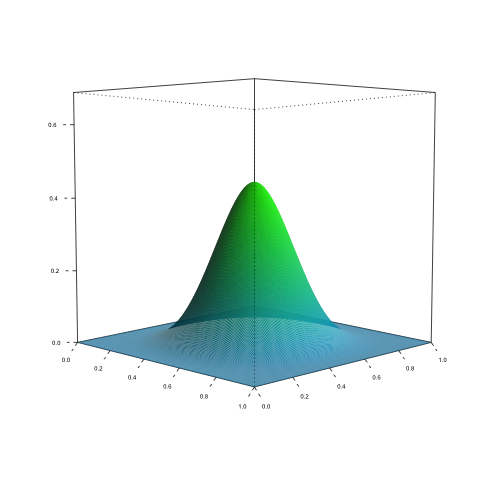
\includegraphics[width=4in, height=4in]{bicubic_bspline.png}
  \caption{Tensor product of two cubic B-splines}\label{bicubic_bspline}
\end{figure}

\begin{figure}[H]
  \centering
  \graphicspath{{img/}}
  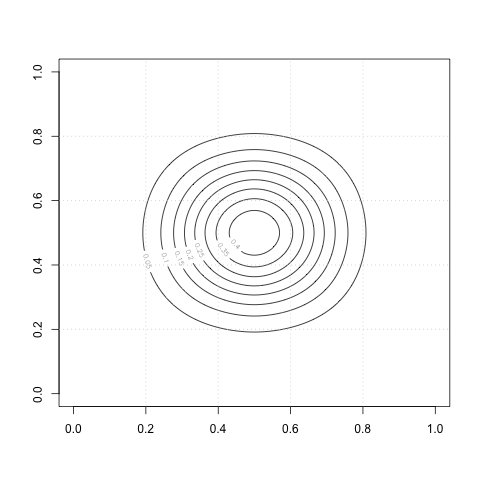
\includegraphics[width=4in, height=4in]{bicubic_bspline_contour.png}
  \caption{Tensor product of two cubic B-splines}\label{bicubic_bspline_contour}
\end{figure}

\subsubsection{{\outlineskeleton P-Splines Regularization}}

\needsparaphrased{The choice of knots has been a subject of much research: too many knots lead to overfitting of the data, too few knots lead to underfitting. Some authors have proposed automatic schemes for optimizing the number and the positions of the knots (Friedman and Silverman, 1989; Kooperberg and Stone, 1991,1992). This is a difficult numerical problem and, to our knowledge, no attractive all-purpose scheme exists.

A different track was chosen by O'Sullivan (1986, 1988). He proposed to use a relatively large number of knots. To prevent overfitting, a penalty on the second derivative restricts the flexibility of the fitted curve, similar to the penalty pioneered for smoothing splines by Reinsch (1967) and that has become the standard in much of the spline literature; see, for example, Eubank (1988), Wahba (1990) and Green and Silverman (1994). \cite{eilers1996flexible} simplify and generalize the approach of O'Sullivan, in such a way that it can be applied in any context where regression on B-splines is useful. Only small modifications of the regression equations are necessary.

The basic idea is not to use the integral of a squared higher derivative of the fitted curve in the penalty, but instead to use a simple difference penalty on the coefficients themselves of adjacent B-splines. We show that both approaches are very similar for second-order differences. In some applications, however, it can be useful to use differences of a smaller or higher order in the penalty. With our approach it is simple to incorporate a penalty of any order in the (generalized)regression equations. A major problem of any smoothing technique is the choice of the optimal amount of smoothing, in our case the optimal weight of the penalty. We use cross-validation and the Akaike information criterion (AIC). In the latter the effective dimension, that is, the effective number of parameters, of a model plays a crucial role. We follow \cite{buja1989linear} in using the trace of the smoother matrix as the effective dimension. Because we use standard regression techniques, this quantity can be computed easily. We find the trace very useful to compare the effective amount of smoothing for different numbers of knots, different degrees of the B-splines and different orders of penalties.}

\subsubsection{{\outlineskeleton P-Splines Penalties for Univariate B-Splines}}

Consider the regression of m data points $\left(x_i,y_i\right)$ on a set of $n$ B-splines $B_j(.)$. The least squares objective function to minimize is

\begin{equation} \label{univariate_bspline_SSE}
\sum_{i=1}^m \left\{ y_i - \sum_{j=1}^n \beta_j B_j\left(x_i\right) \right\}^2
\end{equation}
\noindent
Let the number of knots be relatively large, such that the fitted curve will show more variation than is justified by the data. To make the result less flexible, O'Sullivan (1986, 1988) introduced a penalty on the second derivative of the fitted curve and so formed the objective function

\begin{equation} \label{univariate_bspline_ridge_penalty}
\sum_{i=1}^m \left \{ y_i - \sum_{j=1}^n \beta_j B_j\left(x_i\right) \right \}^2 + \lambda \int_{x_{min}}^{x_{max}} \left\{  \sum_{j=1}^n \beta_j B^{\prime \prime}_j\left(x\right) \right\}^2 \; dx
\end{equation}


The integral of the square of the second derivative of a fitted function has become common as a smoothness penalty, since the seminal work on smoothing splines by Reinsch (1967). There is nothing special about the second derivative; in fact, lower or higher orders might be used as well. In the context of smoothing splines, the first derivative leads to simple equations, and a piecewise linear fit, while higher derivatives lead to rather complex mathematics, systems of equations with a high bandwidth, and a very smooth fit. \cite{eilers1996flexible} propose to base the penalty on (higher-order) finite differences of the coefficients of adjacent B-splines:

\begin{equation} \label{univariate_pspline_diff_penalty}
\sum_{i=1}^m \left \{ y_i - \sum_{j=1}^n \beta_j B_j\left(x_i\right) \right \}^2 + \lambda \sum_{j=k+1}^n \left( \Delta^k \beta_j  \right)^2
\end{equation}

This approach reduces the dimensionality of the problem to n, the number of B-splines, instead of m, the number of observations, with smoothing splines. We still have a parameter A for continuous control over smoothness of the fit. The difference penalty is a good discrete approximation to the integrated square of the $k^{th}$ derivative. What is more important: with this penalty moments of the data are conserved and polynomial regression models occur as limits for large values of A.See Section 5 for details. We will show below that there is a very strong connection between a penalty on second-order differences of the B-spline coefficients and O'Sullivan7s choice of a penalty on the second derivative of the fitted function. However, our penalty can be handled mechanically for any order of the differences.

Difference penalties have a long history that goes back at least to Whittaker (1923); recent applications have been described by Green and Yandell (1985) and Eilers (1989, 1991a, b, 1995).
The difference penalty is easily introduced into the regression equations. That makes it possible to experiment with different orders of the differences. In some cases it is useful to work with even the fourth or higher order. This stems from the fact that for high values of h the fitted curve approaches a parametric (polynomial) model, as will be shown below.
\cite{o1986statistical} used third-degree B-splines and the following penalty:

\begin{equation} \label{osullivan_univariate_bspline_penalty}
h^2 P = \lambda \int_{x_{min}}^{x_max} \left\{ \sum_{j}  \beta_j B_j^{\prime \prime} \left(x, q=3\right) \right\}^2\; dx
\end{equation}
\noindent
From the derivative properties of B-splines it follows that

\begin{equation} \label{osullivan_univariate_bspline_penalty_via_deriv}
h^2 P = \lambda \int_{x_{min}}^{x_max}  \sum_{j} \sum_{k} \Delta^2 \beta_j \Delta^2 \beta_k B_j\left(x,q=1\right)B_k\left(x,q=1\right) dx 
\end{equation}
\noindent
Most of the cross products of $B_j(x; 1)$ and $B_k(x;1)$ vanish as B-splines of degree 1 only overlap when $j$ is $k-1$, $k$, or $k+1$.We thus have that

\begin{align}
h^2 P = {} & \lambda \int_{x_{min}}^{x_{max}} \bigg[ \left\{ \sum_{j}  \Delta^2 \beta_j  B_j\left(x,1\right)  \right\}^2  + 2 \sum_{j}\Delta^2 \beta_j\Delta^2 \beta_{j-1}B_j\left(x,1\right)B_{j-1}\left(x,1\right) \bigg] dx \nonumber \\ 
= {} & \lambda \bigg[ \sum_j \left( \Delta^2\beta_j \right)^2 \int_{x_{min}}^{x_{max}} B_j^2\left(x,1\right)\;dx + 2 \sum_j \Delta^2 \beta_j\Delta^2 \beta_{j-1} \bigg]
\end{align}
\noindent
or
\begin{align}
h^2 P = \lambda \sum_j \left( \Delta^2\beta_j \right)^2 \int_{x_{min}}^{x_{max}} B_j^2\left(x,1\right) dx + {} & 2\lambda \sum_j \Delta^2 \beta_j \Delta^2 \beta_{j-1}  \nonumber \\ 
{} &+\int_{x_{min}}^{x_{max}} B_j\left(x,1\right)B_{j-1}\left(x,1\right) dx
\end{align}
\noindent
which can be written as
\begin{equation}
h^2 P = \lambda\left\{c_1 \sum_j\left( \Delta^2 \beta_j\right)^2 + c_2 \sum_j\Delta^2 \beta_j\Delta^2 \beta_{j-1} \right\}
\end{equation}
\noindent
where, for given equidistant knots, $c_1$ and $c_2$ are constants given by
\begin{equation}
\begin{split}
c_1 & =  \\ \int_{x_{min}}^{x_{max}} B_j^2\left(x,1\right) dx
c_2 & = \int_{x_{min}}^{x_{max}} B_j\left(x,1\right)B_{j-1}\left(x,1\right) dx
\end{split}
\end{equation}



\subsection{Nonparametric approaches to modeling nonlinear time series data}

Zeger and Diggle (1994) present a partially linear model motivated by the longitudinal data produced by the Multicenter AIDS Cohort Study. The data are of the form $\left\{ \left(x_{ij},y_{ij}\left(t_{ij}\right)\right): \;\; j=1,\dots,m_i;\;\;i=1,\dots,n \right\}$, where $x_{ij}$ denotes a $p \times 1$ vector of covariates corresponding to $y_{ij}\left(t_{ij}\right)$, the $j$th measurement on the $i^{th}$ subject at time $t_{ij}$. They let 

\begin{equation} \label{eq:zeger_diggle_VC_model}
Y_{ij}\left(t\right) =  x_{ij}^T\beta + \mu\left(t\right) + W_i\left(t\right) + \epsilon_{ij}
\end{equation}
\noindent
where $\mu\left(t\right)$ is a smooth function of time, and $\beta$ is a $p \times 1$ vector of regression coefficients. The $\left\{ W_i\left(t\right):\;i=1,\dots,n \right\}$ capture the within-subject dependency structure, defined to be independent replicates of a stationary Gaussian process with mean zero and covariance function $\gamma\left(v\right) = \sigma_w^2\rho\left(v, \theta \right)$. The $\left\{ Z_{ij}:\;j=1,\dots,m_i\;i=1,\dots,n \right\}$ are mutually independent Normally distributed error terms with mean zero and variance $\sigma_z^2$.

Hoover, Rice, Wu and Yang (1998) considered the following model:

\begin{equation} \label{eq:hoover_rice_wu_VC_model}
Y\left(t\right) =  \bfX^T\left(t\right)\bfbeta \left(t\right) + \epsilon\left(t\right) 
\end{equation}
\noindent
proposing estimation of the coefficient functions via smoothing splines and local polynomials. $\epsilon\left(t\right)$ is defined as in \ref{eq:zeger_diggle_VC_model} and is assumed to be independent of $\bfX\left(t\right)$. Hoover et al (1998) propose the same model, using smoothing splines and kernel smoothing to estimate  the components of $\bfbeta\left(t\right)$ and develop asymptotic properties of kernel estimators. 



For nonlinear time series applications, Chen \& Tsay \cite{chen1993functional} and Xia \& Li (1999) develop functional-coefficient autoregressive models. The common research in nonlinear time series analysis has focused on several classes of models, such as the threshold autoregressive (TAR) model of Tong (1983, 1990) and the exponential autoregressive (EXPAR) model of Haggan and Ozaki (1981). {\needsparaphrased In this article we are concerned with empirical modeling of nonlinear time series. In particular we focus on exploring the nonlinear feature of a time series in the process of model building. This is achieved by generalizing directly the linear autoregressive (AR) models and exploiting local characteristics of a given time series. The generalized model is referred to as the functional coefficient autoregressive (FAR) models. Most nonlinear AR models considered in the literature are special cases of the FAR model. It turns out that the FAR models are flexible enough to accommodate most nonlinear features considered in the literature while being simple enough to be treated with relative ease. }


\section{Model estimation}

Zeger and Diggle (1994) carry out estimation of $\mu\left(t\right)$ and $\beta$ as defined in model \ref{eq:zeger_diggle_VC_model} iteratively via kernel smoothing and generalized least squares. While more flexible than the classical linear model, this still limiting as it does not allow us to explain any dynamic effect of the covariates over time.  


In the case of a single common smoothing variable, estimation of \ref{eq:VC_mean_function_single_smoothing_covariate} via kernel smoothing is quite straightforward. Since the space of the smoothing variable is of only one dimension, smoothing of the $p$ coefficient functions reduces to finding the local least squares fit using a single smoothing bandwidth. This approach, however, may lead to inadequate estimators since the functions $\beta_0\left(z\right), \beta_1\left(z\right), \dots, \beta_p\left(z\right)$ may need varying degrees of smoothing in the $z$ dimension. To address this, 

\subsection{Kernel estimation with a single smoothing variable}

Suppose we have a random sample of data, consisting of $\left\{ \left(x_1, y_1\right),\dots, \left(x_n, y_n\right)\right\}$, for $i=1,\dots,n$. In classical univariate nonparametric regression, we model 

\begin{equation}
Y_i = f\left(x_i\right) + \epsilon_i,\;\;\;i=1,\dots, n \label{eq:classical_NP_regression_model}
\end{equation} 
\noindent
where $f$ is the unknown smooth regression function of interest, and the $\left\{ \epsilon_i \right\}$ are mutually independent mean-zero errors, with $Var\left(\epsilon_i\right)=\sigma_\epsilon^2$. To derive the form of the estimator of the mean function, we consider expressing $f$ in terms of the joint probability distribution of $X$ and $Y$:

\begin{eqnarray} 
f\left(x\right) = E\left(Y \vert X=x\right) &=& \int yp(y \vert x)\;dy \nonumber \\
&=& \frac{ \int yp(y \vert x)\;dy }{ \int p(y \vert x)\;dy } \label{eq:conditional_mean_y_given_x}
\end{eqnarray}
 
Let $K$ denote a kernel function corresponding to a probability density, $h$ denote the smoothing bandwidth, and let 

\[
K_h\left(t\right) = h^{-1} K\left(h^{-1} t \right)
\] 

The Nadaraya-Watson estimator of the joint density of $x$ and $y$ has form

\begin{eqnarray} 
\hat{p}\left(x,y\right) &=& \frac{1}{nh_x h_y}\sum_{i=1}^{n} K_{h_x}\left(\frac{x-x_i}{h_x}\right) K_{h_y}\left(\frac{y-y_i}{h_y}\right)  \nonumber \\ 
&=& \frac{1}{n}\sum_{i=1}^{n} K_{h_x}\left(x-x_i\right) K_{h_y}\left(y-y_i\right) \label{eq:NW_joint_pdf_estimator} 
\end{eqnarray}
\noindent
Then, substituting \ref{eq:NW_joint_pdf_estimator} for $p\left(x,y\right)$ in the numerator of \ref{eq:conditional_mean_y_given_x}, we can write 

\begin{equation} \nonumber 
\int y \hat{p}\left(x,y\right)\;dy = \frac{1}{n} \int y K_{h_x}\left(x-x_i\right) K_{h_y}\left(y-y_i\right)
\end{equation} 
\noindent
Since $\int yK_{h_y}\left(y-y_i\right)dy = y_i$, we have that 
\begin{equation} \label{eq:num_est}
\int y \hat{p}\left(x,y\right)\;dy = \frac{1}{n}\sum_{i=1}^n K_{h_x}\left(x-x_i\right) y_i 
\end{equation} 
\noindent
Estimating the denominator of \ref{eq:conditional_mean_y_given_x} in similar fashion, we have 

\begin{eqnarray}
\int \hat{p}\left(x,y\right)\;dy &=& \frac{1}{n}\sum_{i=1}^{n} K_{h_x}\left(x-x_i\right) \int K_{h_y}\left(y-y_i\right)\;dy \nonumber \\
&=& \frac{1}{n}\sum_{i=1}^{n} K_{h_x}\left(x-x_i\right) \nonumber \\
&=& \hat{f}_x\left(x\right) \label{eq:den_est} 
\end{eqnarray}

Using \ref{eq:num_est} and \ref{eq:den_est} as plug-in estimators in \ref{eq:conditional_mean_y_given_x}, then 

\begin{equation} 
\hat{f}\left(x\right) = \sum_{i=1}^n W_{h_x}\left(x,x_i\right)y_i
\end{equation}
\noindent
where 
\begin{equation} \nonumber
W_{h_x}\left(x,x_i\right) = \frac{K_{h_x}\left(x-x_i\right) }{\sum_{i=1}^{n} K_{h_x}\left(x-x_i\right)}
\end{equation}
\noindent
and $\sum_{i=1}^n W_{h_x}\left(x,x_i\right) = 1$. One can extend this to the case where the regression function is defined as in \ref{eq:VC_mean_function_single_smoothing_covariate}; the Nadaraya-Watson (NW) estimator of $\bfbeta\left(z_0\right) = \left(\beta_0\left(z_0,\right), \beta_1\left(z_0,\right),\dots,\beta_p\left(z_0,\right)\right)^T$ minimizes

\begin{equation} \nonumber 
\sum_{i=1}^n \left(Y_i - \left(\sum_{j=1}^p \alpha_j X_{ij}\right)\right)^2 K_{h_z}\left(z_0,Z_i\right)
\end{equation} 
\noindent
with respect to $\bfalpha = \left( \alpha_1, \dots, \alpha_p\right)^T$ for each target point $z_0$. Let $\mathcal{X}$ denote the $n \times p$ matrix having $i-j^{th}$ element $X_{ij}$, $\mathcal{W}$ denote the $n \times n$ diagonal matrix with $i^{th}$ diagonal entry $K_{h_z}\left(z_0, Z_i\right)$, and let $\bfZ = \left(Z_1, \dots, Z_n\right)^T$. Further, let $\bfY = \left(Y_1, \dots, Y_n\right)^T$, then the NW estimator has form

\begin{equation} \nonumber
\hat{\bfbeta}\left(z_0\right) = \big[\mathcal{X}^T\mathcal{W}\mathcal{X}\big]^{-1} \mathcal{X}^T\mathcal{W} \bfY
\end{equation} 


It is well known that locally weighted averages can exhibit high bias near the boundaries of the smoothing variable domain, due to the asymmetry of the kernel in that region. This bias can also be present on the interior of the domain when the observed values of $Z$ are irregularly sampled, though it is typically less severe in the interior than near the boundaries. To remedy this, one may consider fitting local linear smoothers, which will correct this bias to first order. The local linear smoother minimizes 

\begin{equation} \label{local_linear_smoother_obj_fun} 
\sum_{i=1}^n \Big[Y_i - \sum_{j=1}^p \left(\alpha_{0j}+\alpha_{1j}\left(Z_i - z_0 \right)\right)X_{ij}\Big]^2 K_{h_z}\left(z_0,Z_i\right)
\end{equation} 
 
 \noindent
 with respect to $\bfalpha_0 = \left( \alpha_{01}, \dots, \alpha_{0p}\right)^T$, and $\bfalpha_1 = \left( \alpha_{11}, \dots, \alpha_{1p}\right)^T$. Let $\mathcal{X}$ denote the $n \times 2p$ matrix having $i-j^{th}$ element $X_{ij}$ and $i-\left(j+p\right)^{th}$ element $\left(Z_i - z_0\right)X_{ij}$ for $1 \le  j \le p$, then the minimizer of \ref{eq:local_linear_smoother_obj_fun} is given by 
 
\begin{equation} \nonumber
\hat{\bfbeta}\left(z_0\right) = \big[ \mathcal{I}_p, \bfO_p \big]\big[\mathcal{X}^T\mathcal{W}\mathcal{X}\big]^{-1} \mathcal{X}^T\mathcal{W} \bfY
\end{equation}   

\noindent
where $\mathcal{I}_p$ is the $p \times p$ identity matrix, and $\bfO_p$ is the $p \times p$ zero matrix. Extensions to the case of a single multivariate smoothing variable $\bfZ$, where the mean function is given by 

\[
E\left(Y \vert \bfX=\bfx, \bfZ=\bfz \right) = x_1\beta_1\left(\bfz\right) + \dots  + x_p\beta_p\left(\bfz\right)
\]
\noindent
However, while boundary effects associated with the NW estimator are a concern in one dimension, the curse of dimensionality makes these effects much more problematic in two or more dimensions. The fraction of points close to the boundary of the domain approaches one as the dimensionality of the input space grows, and simultaneously maintaining locality (and low bias) as well as sizable number of observations in the neighborhood of the target point, $z_0$ (low variance) becomes an increasingly tall order. 

\subsubsection{Kernel bandwidth selection with a single smoothing variable} \label{single_smoothing_var_bandwidth_selection}
\subsubsection{Asymptotic properties of kernel estimators with a single smoothing variable}

\subsubsection{Two-step estimation for multiple bandwidths} \label{two_step_kernel_smoothing}

Model selection as described in \ref{single_smoothing_var_bandwidth_selection} assumes a single smoothing bandwidth $h_z$ as well as a single common kernel function $K$ for every coefficient function $\beta_j$. While convenient and straightforward, in practice, the assumption that each coefficient function should receive the same degree of smoothing is likely to be an erroneous one. Fan and Zhang (1999) present an intuitive formulation of their proposed two-stage estimation procedure that allows for each coefficient function to have its own smoothing bandwidth. Assume that $\beta_p\left(z\right)$ is smoother than the other $p-1$ coefficient functions, and can be locally approximated by a cubic polynomial:

\[
\beta_p\left(z\right) \approx b_{0p} + b_{1p} \left(z-z_0\right) + b_{2p} \left(z-z_0\right)^2 + b_{3p} \left(z-z_0\right)^3
\] 
\noindent 
for any $z_0$ close to $z$. Let $\left\{ \tilde{b}_{0j}, \tilde{b}_{1j} \right\}$, $j=1,\dots, p-1$ and $\tilde{b}_{0p}, \tilde{b}_{1p}, \tilde{b}_{2p}, \tilde{b}_{3p}$ be the minimizers of the weighted sums of squares:

\begin{IEEEeqnarray*}{lll}
\sum_{i=1}^n \Big[ Y_i &-& \sum_{j=1}^{p-1}\left\{ b_{0j} + b_{1j}\left(Z_i-z_0\right) \right\} X_{ij} \\ 
&-& \left\{ b_{0p} + b_{1p} \left(z-z_0\right) + b_{2p} \left(z-z_0\right)^2 + b_{3p} \left(z-z_0\right)^3 \right\} X_{ip} \Big]^2 \times\> K_{h_1}\left(Z_i-z_0\right)
\end{IEEEeqnarray*}

If we take $\tilde{\beta}^{os}_p\left(z_0\right) = \tilde{b}_{0p}$, then they show that the bias of the the \textit{one-step estimator} is $O\left(h_0^2\right)$ and the variance is $O\left( \left(nh_0 \right)^{-1} \right)$. Fan and Zhang (1999) propose a two-step estimation procedure that allows for individual degrees of smoothing of each of the coefficient functions; Cai (2000) further investigated this two-step approach. In the first step, to estimate $\beta_j\left(z_0\right)$, a preliminary estimate, $\tilde{\beta}_j$, is obtained by applying a local cubic smoother to $\beta_j$ and local linear smoothing to the remaining $p-1$ functions with a single common bandwidth, $h_0$, for every $j$. In the second step, a local cubic smoother is again applied to the residuals $Y_i-\sum_{j\ne k} X_{ik} \tilde{\beta}\left( z_0 \right)$ using function-specific bandwidth to obtain the final estimate of $\beta_j\left(z_0\right)$. They present the asymptotic mean-squared error of the estimates obtained by this procedure, and further show  that the estimates achieve optimal convergence rates. Cai (2000) demonstrated that even when every coefficient function exhibits the same degree of smoothness, the two-step estimates exhibit the same asymptotic properties as the usual one-step local smoother.  

\subsection{Kernel estimation with multiple smoothing variables}

A proposed extension of model \ref{eq:VC_mean_function_single_smoothing_covariate} permits each coefficient function to depend on its own smoothing variable: 

\begin{equation} \nonumber
E\left(Y \vert \bfX=\bfx,\;Z = z \right) = x_1\beta_1\left(z_1\right) + \dots  + x_p\beta_p\left(z_p\right)
\end{equation}

While the expression of the model itself does not make this obvious, estimation of this model is significantly different than the estimation of the model assuming a single common smoothing parameter for every coefficient function. Xue \& Yang (2006a) further generalized this model where each coefficient function is replaced by a multivariate function with additive structure:

\begin{equation} \label{eq:VC_mean_MV_function_multiple_smoothing_covariates}
E\left(Y \vert \bfX=\bfx,\;\bfZ = \bfz \right) = x_1\sum_{j=1}^q \beta_{1j}\left(z_1\right) + \dots  + x_p\sum_{j=1}^q \beta_{pj}\left(z_p\right)
\end{equation}
\noindent
which allows for inclusion of all interaction terms $X_j \beta_{jk}\left(Z_k\right)$, $j=1,\dots,p$, $k=1,\dots, q$. Applying multivariate kernel smoothing locally to each point $\bfz = \left(z_1,\dots,z_p \right)^T$ results in multivariate functions of the entire covariate vector, losing the structure of model \ref{eq:VC_mean_function_multiple_smoothing_covariates}. To extract proper estimates of the $\left\{  \beta_j \right\}$, two primary methodologies have been proposed: marginal integration and smooth backfitting. Linton and Nielsen (1995) employ local kernel smoothing to estimate the multivariate coefficient functions $\left\{ \beta_j\left( \bfz\right) \right\}$, minimizing

\[
n^{-1} \sum_{i=1}^n \left( Y_i  - \sum_{j=1}^q \alpha_j X_{ij} \right)^2 K_{h_1}\left(z_1,Z_{i1}\right) \times \dots \times K_{h_p}\left(z_p,Z_{ip}\right)
\]
\noindent
for each value of $\bf$. Integrating the multivariate coefficient functions over the support of the smoothing variables gives marginal estimates of $\beta_j$. This approach, however, suffers from the curse of dimensionality, as the attractive statistical properties of the estimators $\hat{\beta}_j$ depend heavily on the consistency of the $\left\{ \alpha_j \right\}$, which requires $n\times h_1\times \dots \times h_p \rightarrow \infty$, thus losing the attractive qualities of local methods. The smooth backfitting method initially introduced by Mammen et al. (1999) for additive regression models enjoys both theoretical and numerical advantages over the integration method, and is free of the curse of dimensionality. To estimate $\left\{ \alpha_j \right\}$, one minimizes the integrated weighted sum of squares

\[
\int n^{-1} \sum_{i=1}^n \left( Y_i - \sum_{j=1}^p \alpha_j\left(z_j\right) \right)^2 K_{h_1}\left(z_1,Z_{i1}\right) \times \dots \times K_{h_p}\left(z_p,Z_{ip}\right) \;d\bfz
\]
\noindent
over the space of function tuples $\mathcal{H} = \left\{ \bfalpha = \left(\alpha_1,\dots, \alpha_p\right):\alpha_j\left(\bfz\right) = \alpha_j\left(z_j\right) \right\}$, so that the optimization must not be performed for every $\bfz$. For a detailed discussion of these methods, we refer the reader to Linton and Nielsen (1995) and Mammen \& Park (2005). 





\subsection{Basis expansions and penalized likelihood techniques} \label{VC_spline_models}

In classical nonparametric regression problems, $m\left(x\right) = E\left(Y\vert X\right)$ is represented by a linear basis expansion in $X$, so that

\[
E\left(Y \vert X\right) = \sum_{j=1}^M \beta_m b_m\left(X\right)
\]
\noindent
with $M \rightarrow \infty$. The general estimation framework may be described as follows: The estimation space, $G = G_n$, is the linear space of bounded functions having finite dimension $M_n$. For a given loss function $\mathcal{L}$, the estimate of $m$, $\hat{m}$, is defined to be the element of $G_n$ which minimizes $\mathcal{L}$ and maybe be characterized by the estimates of the basis function coefficients $\beta_1,\dots, \beta_m$. It is typical that the true mean function does not belong to $G_n$, and members of $G_n$ are taken to be an approximation to the truth. Typical choices for loss functions include sums of squared errors or negative log likelihood functions. To this end, it is natural to allow the dimension of the estimation space to grow with the sample size. The choice of basis is not a trivial one, and some choices include logarithms, power functions, or wavelets; there is, however, disadvantages to using basis functions with unrestricted support. Piecewise polynomials and splines are families of functions with each member of which having bounded support. This allows for local representations of $m\left(x\right)$, while still permitting ease of implementation, as their estimation is carried out through the global optimization of $\mathcal{L}$. 

These methods in the classical setting have been explored extensively; Chen (2007) provides an extensive review of the asymptotic behaviour of these estimators. Zhou, Shen, and Wolfe (1998) establish asymptotic normality of univariate regression splines; they present explicit expressions for the asymptotic pointwise bias and variance of the estimator, providing a method of constructing confidence intervals and confidence regions when the knots are asymptotically equally spaced and are distributed according to a continuous density. Their results additionally require that the order of the spline is equal to the order of the derivative of the unknown function to be estimated. Huang et al. (2003) establish asymptotic results for not only the univariate case, but also for tensor product splines and multivariate splines on triangulations.  

A general representation of models \ref{eq:VC_mean_function_single_smoothing_covariate}, \ref{eq:VC_mean_function_multiple_smoothing_covariates}, and \ref{eq:VC_mean_MV_function_multiple_smoothing_covariates} may be represented as follows:

\begin{equation} \label{eq:general_VC_model}
E\left(Y \vert \bfX, \bfZ\right) = \sum_{i=1}^q \bfX_i^T \bfbeta_i\left(\bfZ_i\right)
\end{equation}
\noindent
where $\bfX_i$ is a $d_i \times 1$ vector, $d_i \ge 1$; $\bfX$ is the collection of all covariates contained in $\left\{ \bfX_i \right\}$, $i=1,\dots,q$. For example, model \ref{eq:VC_mean_MV_function_multiple_smoothing_covariates} may be written as above by letting $\bfX_i \equiv \bfX = \left(X_1,\dots, X_p\right)^T$ for every $j$. The majority of the work in this area has been for the case where $q=1$.  Xue and Yang (2005a) allowed for multivariate coefficient functions, assuming an additive structure by letting

\begin{eqnarray} 
E\left(Y \vert \bfX, \bfZ\right) &=& \sum_{i=1}^{d_1} X_i \beta_i\left(\bfZ\right) \label{eq:xue_VC_model}\\
\beta_i\left(\bfZ\right) &=& \sum_{j=1}^{d_2} \beta_{ij}\left(Z_j\right) \nonumber
\end{eqnarray}
\noindent
for $i=1,\dots, d_1$.

 

















\subsection{Smoothing methods with longitudinal data}

Models \ref{eq:VC_mean_function_single_smoothing_covariate}, \ref{eq:VC_mean_function_multiple_smoothing_covariates}, and \ref{eq:VC_mean_MV_function_multiple_smoothing_covariates} can be written as follows:

\begin{equation} \label{eq:functional_VC_model}
Y\left(t\right) = \sum_{j=1}^q \bfX_j^T \bff \left(T\right) + \epsilon\left(T\right)
\end{equation}

where $\bff = \left(f_1,\dots, f_q \right)^T$ is the vector of coefficient functions of interest and $\epsilon\left(t\right)$ is a mean zero stochastic process. Both the response and covariates are assumed to be observed at subject-specific times, which may be irregularly spaced. Let $\bfX_{ij} = \bfX_i\left(T_{ij}\right)$ and $Y_{ij} = Y_i\left(T_{ij}\right)$ denote the observed covariates and responses on subject $i$ at random time points $\left\{ T_{ij} \right\}$, $j=1,\dots,n_i$. Given this structure, model  \ref{eq:functional_VC_model} can be written 
   
\begin{equation} \label{longitudinal_VC_model}
Y_{ij} = \bff\left(T_{ij}\right)^T\bfX_{ij} + \epsilon_{ij}
\end{equation}
\noindent
where $\epsilon_{ij} = \epsilon\left(T_{ij}\right)$. The $\left\{ T_{ij} \right\}$ are assumed to be independent for all $i,j$; $\bfX_{ij}$ and $\epsilon_{ij}$ are assumed to be independent across values of $i$, but may exhibit within-subject dependency structure.  A simple avenue of model estimation for model \ref{eq:longitudinal_VC_model} is to apply local smoothing, where the Nadaraya-Watson estimator minimizes 

\begin{equation} \label{eq:longitudinal_NW_objective_function}
N^{-1} \sum_{i=1}^{n} \sum_{j=1}^{n_i} \left(Y_{ij} - \sum_{k=1}^q \alpha_k X_{ijk} \right)^2 K_h\left(t,T_{ij}\right)
\end{equation}
\noindent

with respect to $\alpha = \left(\alpha_1,\dots, \alpha_q \right)^T$, where $N = \sum_{i=1}^n n_i$. The specification in \ref{eq:longitudinal_NW_objective_function} places equal weights on all subjects; to assign individual weights to each subject's contribution to the loss function, one may instead minimize

\begin{equation} \label{eq:longitudinal_NW_objective_function}
n^{-1} \sum_{i=1}^{n} w_i \sum_{j=1}^{n_i} \left(Y_{ij} - \sum_{k=1}^q \alpha_k X_{ijk} \right)^2 K_h\left(t,T_{ij}\right)
\end{equation}
\noindent 
where one may specify, for example, $w_i = n_i^{-1}$. Hoover et al. (1998) proposed kernel estimation using local polynomial smoothing, of which the minimization of \ref{eq:longitudinal_NW_objective_function} is a special case. Wu et al present the construction of both point-wise confidence intervals as well as simultaneous confidence regions based on the asymptotic normality of the local kernel smoother.

\bibliography{Master} 
%\bibliographystyle{amsplain}
\bibliographystyle{apalike}


\end{document}

